%describe how you evaluated to show that your approach was successful. You may need a methods section, a results section and a conclusion

This chapter reflects on the theoretical architecture (see Figure \ref{fig:wrtc-enterprise-gateway}) drafted in the integration section of the previous chapter. I will compare my model against a study 3GPP\footnote{http://www.3gpp.org/} did on giving \gls{wrtc} clients access to \gls{ims}, which is similar to this case. Then I will discuss the results and derive some guidelines.


\section{Evaluate against criteria defined by 3GPP}
There is an ongoing effort at the 3GPP on giving \gls{wrtc} clients access to \gls{ims} with 3GPP TR 23.701\cite{3gpp-wrtc-access-ims} as the current proposed architecture. \gls{ims} is basically an architectural framework for delivering IP multimedia services. It was originally designed for evolving mobile networks beyond \gls{gsm}. Later it has evolved to include Wireless LAN and fixed lines, it's intended to aid the access of multimedia and voice applications across different networks. This study is relevant because most telecom companies already have IMS or a similar architecture in place for doing real-time communication. The following diagram shows the proposed architecture:

\begin{figure}[here]
\centerline{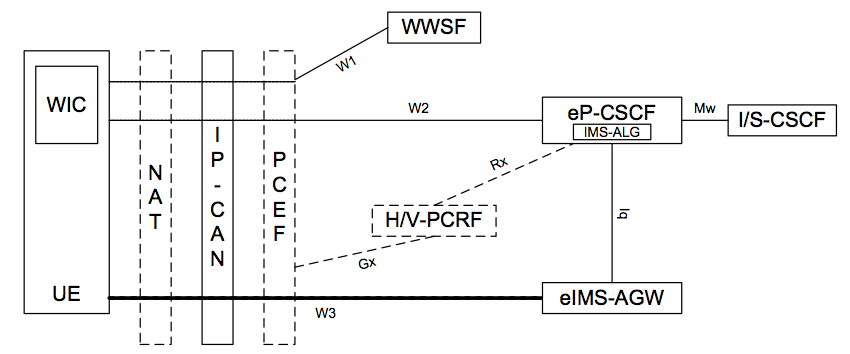
\includegraphics[scale=0.5]{3gpp-wrtc-ims-architecture.png}}
\caption{WebRTC IMS architecture by 3GPP TR 23.701 as work in progress.}
\label{fig:wrtc-ims-architecture}
\end{figure}

Let's look at the main elements:

\textbf{WebRTC IMS Client (WIC)}
is downloaded from the WWSF. It provides the application logic and \gls{wrtc} API calls to access the communication services of \gls{ims}. It works on any device supporting a browser that supports \gls{wrtc}. This is basically the same component as the mobile client in the previous chapter.

\textbf{User Equipment(UE)}
is a device or application. It can be a web application running in a browser, a tablet or mobile phone.

\textbf{WebRTC Web Server Function (WWSF)}
is from where the client is downloaded. This could be a web server hosting the WIC, or an app store such as Google Play.

\textbf{P-CSCF enhanced for WebRTC (eP-CSCF)}
is the entry point of SIP requests. They propose to receive SIP over WebSockets. This is essentially the signaling gateway. It adapts signaling on the \gls{wrtc} side to standard IMS-SIP. The specification is open to the use of different protocols, but this is the proposed solution.

\textbf{IMS Access Gateway enhanced for WebRTC (eIMS-AGW)}
supports \gls{rtcweb} media as defined by \gls{ietf}. This would be similar to my transport proxy gateway function. It needs to support these functions:
\begin{itemize}
\item{SRTP-DTLS. \gls{sdes} is what's used in \gls{ims}}
\item{Audio/video transcoding. H.264 is the \gls{ims} standard}
\item{RTCP demultiplexing. \gls{rtcweb} supports multiplexing of audio/video calls and RTP/RTCP over same RTP session and port. This is not supported in \gls{ims}, so this component needs to support demultiplexing.}
\end{itemize}

In addition this component must also support negotiating ICE candidates including STUN and TURN.

\textbf{IP Connectivity Access Network (IP-CAN)}
is used to reach the IMS core from the UE. Can be LTE\footnote{Long-Term Evolution is a standard for wireless communication of high-speed data for mobile phones.} for mobile, DSL or WLAN.

\textbf{Policy and Charging Rules Function (PCRF) and Policy and Charging Enforcement Function (PCEF)}
supports policy and charging control decisions based on session and media-related information obtained from the P-CSCF. It uses deep packet inspection and decides based on rules whether the traffic is allowed or not. This is similar to a \gls{dmz} mentioned in earlier chapters.

\textbf{Network Address Translation (NAT)}
the WIC would normally be behind a NAT element, so a box has been included in the diagram. ICE is used to enable two-way flows of SRTP behind NAT, therefore a media gateway needs to have ICE implemented to exchange media flows with the \gls{ims} core.

\section{Results}
Looking at the similarities of the gateway proposed in this thesis together with the one proposed by the 3GPP, they both look very similar in nature, with some added thoughts around the firewall issue present in enterprise systems in ours. In the next chapter I will discuss the findings in this thesis and look at future improvements.